\documentclass[a4paper, 9pt]{scrartcl}\usepackage[]{graphicx}\usepackage[]{xcolor}
% maxwidth is the original width if it is less than linewidth
% otherwise use linewidth (to make sure the graphics do not exceed the margin)
\makeatletter
\def\maxwidth{ %
  \ifdim\Gin@nat@width>\linewidth
    \linewidth
  \else
    \Gin@nat@width
  \fi
}
\makeatother

\definecolor{fgcolor}{rgb}{0.345, 0.345, 0.345}
\newcommand{\hlnum}[1]{\textcolor[rgb]{0.686,0.059,0.569}{#1}}%
\newcommand{\hlstr}[1]{\textcolor[rgb]{0.192,0.494,0.8}{#1}}%
\newcommand{\hlcom}[1]{\textcolor[rgb]{0.678,0.584,0.686}{\textit{#1}}}%
\newcommand{\hlopt}[1]{\textcolor[rgb]{0,0,0}{#1}}%
\newcommand{\hlstd}[1]{\textcolor[rgb]{0.345,0.345,0.345}{#1}}%
\newcommand{\hlkwa}[1]{\textcolor[rgb]{0.161,0.373,0.58}{\textbf{#1}}}%
\newcommand{\hlkwb}[1]{\textcolor[rgb]{0.69,0.353,0.396}{#1}}%
\newcommand{\hlkwc}[1]{\textcolor[rgb]{0.333,0.667,0.333}{#1}}%
\newcommand{\hlkwd}[1]{\textcolor[rgb]{0.737,0.353,0.396}{\textbf{#1}}}%
\let\hlipl\hlkwb

\usepackage{framed}
\makeatletter
\newenvironment{kframe}{%
 \def\at@end@of@kframe{}%
 \ifinner\ifhmode%
  \def\at@end@of@kframe{\end{minipage}}%
  \begin{minipage}{\columnwidth}%
 \fi\fi%
 \def\FrameCommand##1{\hskip\@totalleftmargin \hskip-\fboxsep
 \colorbox{shadecolor}{##1}\hskip-\fboxsep
     % There is no \\@totalrightmargin, so:
     \hskip-\linewidth \hskip-\@totalleftmargin \hskip\columnwidth}%
 \MakeFramed {\advance\hsize-\width
   \@totalleftmargin\z@ \linewidth\hsize
   \@setminipage}}%
 {\par\unskip\endMakeFramed%
 \at@end@of@kframe}
\makeatother

\definecolor{shadecolor}{rgb}{.97, .97, .97}
\definecolor{messagecolor}{rgb}{0, 0, 0}
\definecolor{warningcolor}{rgb}{1, 0, 1}
\definecolor{errorcolor}{rgb}{1, 0, 0}
\newenvironment{knitrout}{}{} % an empty environment to be redefined in TeX

\usepackage{alltt}
\usepackage[ngerman]{babel}
% -----------------------------------------------------------------------

% -----------------------------------------------------------------------
%% ------------------------------------------------------------
%% by J.Kruppa on Friday, February 11, 2022 (11:31)
%% \def\mainDir{\Sexpr{exam_path}}
\def\source{/Users/jokruppa/source/tex}
\usepackage[margin=2cm, includefoot]{geometry}
\setlength{\parindent}{0cm}
\usepackage{booktabs}
\usepackage{amsmath}
\usepackage{scalerel,amssymb}
\usepackage{setspace}
\def\csquare{{\Large $\boxtimes$}}
\def\msquare{{\Large $\square$}}
\usepackage[normalem]{ulem}
\usepackage{array}
\usepackage{xcolor}
\usepackage{float}
\usepackage{currfile}
\usepackage{tikz}
\usepackage[nomessages]{fp}

%% beamer defs
\def\lecture{Klausurfragen der Bio Data Science}

%% exam defs
\def\examtitle{\lecture}
\def\exammodule{
\vspace{-1.75cm}  
\begin{graybox}{}
\vspace{2Ex}
\textbf{\large Name:} \rule[0ex]{16.75em}{.4pt}
\hfill \textnormal{\textit{Nicht bestanden:}} \msquare \\[2.5Ex]
\textbf{\large Vorname:} \rule[0ex]{15em}{.4pt} \\[2.5Ex]
\textbf{\large Matrikelnummer:} \rule[0ex]{10.8em}{.4pt}
\hfill Endnote: \rule[0ex]{7em}{.4pt} 
\end{graybox}
\vspace{3Ex}
\phantom{text}
}
\def\examsemester{Sommersemester \& Wintersemester}
\def\examdate{\today}
%% ------------------------------------------------------------
\definecolor{darkblue}{rgb}{0,0,.5}
\definecolor{darkpurple}{rgb}{0.4117, 0.2, 0.4117}
\definecolor{uni}{rgb}{0,0.3137,0.6078}
\definecolor{gray}{gray}{0.7}

\usepackage{tcolorbox}
\definecolor{logo1}{RGB}{0, 158, 227}
\definecolor{gray5}{RGB}{247, 247, 247}
\definecolor{gray2}{RGB}{102, 102, 102}

\newtcolorbox{graybox}[1]{
  colback=gray5,%%red!5!white,
  colframe=gray2,%%red!75!black,
  fonttitle=\bfseries\Large,
  %%valign=center,
  fontupper=\large,
  before skip=10pt plus 2pt,
  after skip=20pt plus 4pt,
  title=#1}

\newtcolorbox{takehomebox}[1]{
  colback=gray5,%%red!5!white,
  colframe=logo1,%%red!75!black,
  fonttitle=\bfseries\Large,
  %%valign=center,
  fontupper=\large,
  before skip=10pt plus 2pt,
  after skip=10pt plus 2pt,
  title=#1}

\def\Rlogo{
\includegraphics[width = 0.5cm]{\string~/Documents/GitHub/exam/img/Rlogo}\;}

\usepackage[scaled=.90]{helvet} 
\usepackage{fancyhdr}
\usepackage{lastpage}
\usepackage{hyperref}
\hypersetup{
    colorlinks=true,       % false: boxed links; true: colored links
    linkcolor=black,          % color of internal links 
    urlcolor=magenta           % color of external links
}
\renewcommand{\familydefault}{\sfdefault}

\title{
\large \exammodule \\[5Ex]
\Huge \examtitle \\[2Ex] 
\Large Hochschule Osnabr{\"u}ck
}
\author{Pr{\"u}fer: Prof. Dr. Jochen Kruppa \\
Fakult{\"a}t f{\"u}r Agrarwissenschaften und Landschaftsarchitektur \\ 
j.kruppa@hs-osnabrueck.de}
\date{Version vom \examdate}

%% ------------------------------------------------------------
%% by J.Kruppa on Tuesday, September 23, 2014 (12:50)
%% Header
\renewcommand{\headrulewidth}{0pt}
\renewcommand{\footrulewidth}{0pt}
\pagestyle{fancy}

\fancyhf{}
\fancyhead[L]{}
\fancyhead[R]{}
\fancyfoot[R]{\thepage}
\fancyfoot[L]{\footnotesize \examtitle}

\fancypagestyle{empty}{
 \fancyhf{}
 \fancyhead[L]{}
 \fancyhead[R]{}
 \fancyfoot[R]{\thepage}
 \fancyfoot[L]{\footnotesize \examtitle}
}

\usepackage{arevtext,arevmath}

\newcommand\Tstrut{\rule{0pt}{2.6ex}}         % = `top' strut
\newcommand\Bstrut{\rule[-0.9ex]{0pt}{0pt}}   % = `bottom' strut
\def\strut{\Tstrut\Bstrut}

% -----------------------------------------------------------------------
\IfFileExists{upquote.sty}{\usepackage{upquote}}{}
\begin{document}
% -----------------------------------------------------------------------
\maketitle
\thispagestyle{empty}
\clearpage
% -----------------------------------------------------------------------

\begin{graybox}{Erlaubte Hilfsmittel f{\"u}r die Klausur}
  \vspace{1Ex}
  \begin{itemize}
  \item Normaler Taschenrechner ohne M{\"o}glichkeit der Kommunikation mit anderen
    Ger{\"a}ten - also ausdr{\"u}cklich kein Handy!
  \item Eine DIN A4-Seite als beidseitig, selbstgeschriebene,
    handschriftliche Formelsammlung - keine digitalen Ausdrucke. 
  \item \textbf{You can answer the questions in English without any consequences.}  
  \end{itemize}
\end{graybox}
\vfill

\begin{graybox}{Ergebnis der Klausur}
  \vspace{1Ex}
  \begin{itemize}
  \item[] \rule[0ex]{3em}{.4pt}\, von 20\, Punkten sind aus dem Multiple
    Choice Teil erreicht.
  \item[] \rule[0ex]{3em}{.4pt}\, von 67 Punkten sind aus dem Rechen- und
    Textteil erreicht. 
  \item[] \rule[0ex]{3em}{.4pt}\, von 87 Punkten in Summe.
  \item[] Es wird folgender Notenschl{\"u}ssel angewendet.   
  \end{itemize}
  \vspace{1ex}
\begin{center}
  \begin{tabular}[c]{cc}
    \toprule
    \textbf{Punkte}	&	\textbf{Note}	\\
    \midrule
    83.0 - 87.0	&	1,0	\\
    79.0 - 82.5	&	1,3	\\
    74.5 - 78.5	&	1,7	\\
    70.5 - 74.0	&	2,0	\\
    66.0 - 70.0	&	2,3	\\
    61.5 - 65.5	&	2,7	\\
    57.5 - 61.0	&	3,0	\\
    53.0 - 57.0	&	3,3	\\
    49.0 - 52.5	&	3,7	\\
    43.5 - 48.5	&	4,0	\\
    \bottomrule
  \end{tabular}
\end{center}
  \vspace{1ex}
\begin{itemize}
\item[] Es ergibt sich eine Endnote von \rule[0ex]{4em}{.4pt}.
\end{itemize}
  \vspace{1Ex}
\end{graybox}

% -----------------------------------------------------------------------
\newpage
% -----------------------------------------------------------------------

\begin{graybox}{Multiple Choice Aufgaben}
  \begin{itemize}
  \item Pro Multipe Choice Frage ist \emph{genau} eine Antwort richtig.
  \item \textbf{Übertragen Sie Ihre Kreuze in die Tabelle auf
      dieser Seite.}
  \item Es werden nur Antworten berücksichtigt, die in dieser Tabelle
    angekreuzt sind!
  \end{itemize}

\begin{center}
  \large
  \begin{tabular}{|r|c|c|c|c|c||c|}
    \hline
    & \textbf{A} & \textbf{B} & \textbf{C} & \textbf{D} & \textbf{E} & $\boldsymbol{\checkmark}$\strut\\
    \hline
    1 Aufgabe &   &   &   &   &   & \strut\\
    \hline
    2 Aufgabe &   &   &   &   &   & \strut\\
    \hline
    3 Aufgabe &   &   &   &   &   & \strut\\
    \hline
    4 Aufgabe &   &   &   &   &   & \strut\\
    \hline
    5 Aufgabe &   &   &   &   &   & \strut\\
    \hline
    6 Aufgabe &   &   &   &   &   & \strut\\
    \hline
    7 Aufgabe &   &   &   &   &   & \strut\\
    \hline
    8 Aufgabe &   &   &   &   &   & \strut\\
    \hline
    9 Aufgabe &   &   &   &   &   & \strut\\
    \hline
    10 Aufgabe &   &   &   &   &   & \strut\\
    \hline
  \end{tabular}
\end{center}

\begin{itemize}
\item Es sind \rule[0ex]{2em}{.4pt}\, von 20 Punkten erreicht worden.
\end{itemize}
\end{graybox}

\vfill

\begin{graybox}{Rechen- und Textaufgaben}
  \begin{itemize}
  \item Die Tabelle wird vom Dozenten ausgefüllt.
  \end{itemize}
  \begin{center}
    \large
    \begin{tabular}{|l|c|c|c|c|c|c|c|}
      \hline
      \textbf{Aufgabe} & 11 & 12 & 13 & 14 & 15 & 16 & 17 \strut\\
      \hline
      \textbf{Punkte} & 
      \hspace{1Ex}\Large\textcolor{gray!70}{10}\hspace{1Ex}  & 
      \hspace{1Ex}\Large\textcolor{gray!70}{8}\hspace{1Ex}  & 
      \hspace{1Ex}\Large\textcolor{gray!70}{13}\hspace{1Ex}  & 
      \hspace{1Ex}\Large\textcolor{gray!70}{7}\hspace{1Ex}  & 
      \hspace{1Ex}\Large\textcolor{gray!70}{10}\hspace{1Ex}  & 
      \hspace{1Ex}\Large\textcolor{gray!70}{10}\hspace{1Ex}  & 
      \hspace{1Ex}\Large\textcolor{gray!70}{9}\hspace{1Ex} \strut\\
      \hline
  \end{tabular}
\end{center}
\begin{itemize}
\item Es sind \rule[0ex]{2em}{.4pt}\, von 67 Punkten erreicht worden.
\end{itemize}
\end{graybox}

% -----------------------------------------------------------------------
\clearpage
% -----------------------------------------------------------------------


\section{Aufgabe \hfill (2 Punkte)}

Die Randomisierung von Beobachtungen bzw. Samples zu den Versuchseinheiten
ist bedeutend in der Versuchsplanung. Welche der folgenden Aussagen ist richtig?



\begin{enumerate}
\item [\textbf{A} \msquare] Randomisierung bringt starke Unstrukturiertheit in das Experiment und erlaubt erst von der Stichprobe auf die Grundgesamtheit zur{"u}ckzuschliessen.
\item [\textbf{B} \msquare] Randomisierung erlaubt erst die Varianzen zu sch{"a}tzen. Ohne eine Randomisierung ist die Berechnung von Mittelwerten und Varianzen nicht m{"o}glich.
\item [\textbf{C} \msquare] Randomisierung erlaubt erst die Mittelwerte zu sch{"a}tzen. Ohne Randomisierung keine Mittelwerte.
\item [\textbf{D} \msquare] Randomisierung sorgt f{"u}r Strukturgleichheit und erlaubt erst von der Stichprobe auf die Grundgesamtheit zur{"u}ckzuschliessen.
\item [\textbf{E} \msquare] Randomisierung war bis 1952 bedeutend, wurde dann aber in Folge besserer Rechnerleistung nicht mehr verwendet. Aktuelle Statistik nutzt keine Randomisierung mehr.
\end{enumerate} 

\section{Aufgabe \hfill (2 Punkte)}



Sie haben folgende unadjustierten p-Werte gegeben: 0.89, 0.34, 0.21, 0.01 und 0.02. Sie adjustieren die p-Werte nach
Bonferroni. Welche Aussage ist richtig?



\begin{enumerate}
\item [\textbf{A} \msquare] Nach der Bonferroni-Adjustierung ergeben sich die adjustierten p-Werte von 1, 1, 1, 0.05 und 0.1. Die adjustierten p-Werte werden zu einem $\alpha$-Niveau von 5\% verglichen.
\item [\textbf{B} \msquare] Nach der Bonferroni-Adjustierung ergeben sich die adjustierten p-Werte von 0.178, 0.068, 0.042, 0.002 und 0.004. Die adjustierten p-Werte werden zu einem $\alpha$-Niveau von 1\% verglichen.
\item [\textbf{C} \msquare] Nach der Bonferroni-Adjustierung ergeben sich die adjustierten p-Werte von 4.45, 1.7, 1.05, 0.05 und 0.1. Die adjustierten p-Werte werden zu einem $\alpha$-Niveau von 5\% verglichen.
\item [\textbf{D} \msquare] Nach der Bonferroni-Adjustierung ergeben sich die adjustierten p-Werte von 0.178, 0.068, 0.042, 0.002 und 0.004. Die adjustierten p-Werte werden zu einem $\alpha$-Niveau von 5\% verglichen.
\item [\textbf{E} \msquare] Nach der Bonferroni-Adjustierung ergeben sich die adjustierten p-Werte von 1, 1, 1, 0.05 und 0.1. Die adjustierten p-Werte werden zu einem $\alpha$-Niveau von 1\% verglichen.
\end{enumerate} 

\section{Aufgabe \hfill (2 Punkte)}

Nach einem Experiment mit f{\"u}nf Weizensorten ergibt eine ANOVA ($p = 0.041$)
einen signifikanten Unterschied f{\"u}r den Ertrag. Sie f{\"u}hren anschlie{\ss}end die
paarweisen t-Tests f{\"u}r alle Vergleiche der verschiedenen Weizensorten
durch. Nach der Adjustierung f{\"u}r multiples Testen ist kein p-Wert unter der
$\alpha$-Schwelle. Sie schauen sich auch die rohen, unadjustierten p-Werte
an und finden hier als niedrigsten p-Wert $p_{3-2} = 0.053$. Welche Aussage
ist richtig? 



\begin{enumerate}
\item [\textbf{A} \msquare] Die ANOVA testet auf der gesamten Fallzahl. Die einzelnen t-Tests immer nur auf einer kleineren Subgruppe. Da mit weniger Fallzahl weniger signifikante Ergebnisse zu erwarten sind, kann eine Diskrepenz zwischen der ANOVA und den paarweisen t-Tests auftreten.
\item [\textbf{B} \msquare] Die ANOVA testet auf der gesamten Fallzahl. Es w{"a}re besser die ANOVA auf der gleichen Fallzahl wie die einzelnen t-Tests zu rechnen.
\item [\textbf{C} \msquare] Der Fehler liegt in den t-Tests. Wenn eine ANOVA signifikant ist, dann muss zwangsweise auch ein t-Test signifikant sein.
\item [\textbf{D} \msquare] Es gibt einen Fehler in der Varianzstruktur. Daher kann die ANOVA nicht richtig sein und paarweise t-Tests liefern das richtige Ergebnis.
\item [\textbf{E} \msquare] Die adjustierten p-Werte deuten in die richtige Richtung. Zusammen mit den nicht signifikanten rohen p-Werten ist von einem Fehler in der ANOVA auszugehen.
\end{enumerate} 

\section{Aufgabe \hfill (2 Punkte)}




Berechnen Sie den Median, das $1^{st}$ Quartile sowie das $3^{rd}$ Quartile von $y$ mit 10, 22, 8, 13, 17, 12 und 51.



\begin{enumerate}
\item [\textbf{A} \msquare] Es ergibt sich 13 +/- 22
\item [\textbf{B} \msquare] Es ergibt sich 13 [10, 22]
\item [\textbf{C} \msquare] Es ergibt sich 19 [11, 23]
\item [\textbf{D} \msquare] Es ergibt sich 19 +/- 10
\item [\textbf{E} \msquare] Es ergibt sich 13 +/- 10
\end{enumerate} 

\section{Aufgabe \hfill (2 Punkte)}



Sie f{\"u}hren ein Feldexperiment durch um das Gewicht von Maiss zu
steigern. Die Pflanzen wachsen unter einer Kontrolle und zwei verschiedenen
Behandlungsbedingungen. Nach der Berechnung einer einfaktoriellen ANOVA
ergibt sich ein $\eta^2 = 0.22$. Welche Aussage ist richtig?



\begin{enumerate}
\item [\textbf{A} \msquare] Das $\eta^2$ ist die Korrelation der ANOVA. Mit der Ausnahme, dass 0 der beste Wert ist.
\item [\textbf{B} \msquare] Das $\eta^2$ beschreibt den Anteil der Varianz, der von den Behandlungsbedingungen nicht erkl{"a}rt wird. Somit der Rest an nicht erkl{"a}rbarer Varianz.
\item [\textbf{C} \msquare] Das $\eta^2$ ist ein Wert f{"u}r die G{"u}te der ANOVA. Je kleiner desto besser. Ein $\eta^2$ von 0 bedeutet ein perfektes Modell mit keiner Abweichung. Die Varianz ist null.
\item [\textbf{D} \msquare] Das $\eta^2$ beschreibt den Anteil der Varianz, der von den Behandlungsbedingungen erkl{"a}rt wird. Das $\eta^2$ ist damit mit dem $R^2$ aus der linearen Regression zu vergleichen.
\item [\textbf{E} \msquare] Die Berechnung von $\eta^2$ ist ein Wert f{"u}r die Interaktion.
\end{enumerate} 

\section{Aufgabe \hfill (2 Punkte)}

Welche Aussage {\"u}ber den t-Test im Allgmeinen ist richtig? 



\begin{enumerate}
\item [\textbf{A} \msquare] Der t-Test testet generell zu einem erh{"o}hten $\alpha$-Niveau von 20\%.
\item [\textbf{B} \msquare] Der t-Test ist ein Vortest der ANOVA und basiert daher auf dem Vergleich von Streuungsparametern
\item [\textbf{C} \msquare] Der t-Test vergleicht die Mittelwerte von zwei Gruppen unter der strikten Annahme von Varianzhomogenit{"a}t. Sollte keine Varianzhomogenit{"a}t vorliegen, so gibt es keine M{"o}glichkeit den t-Test in einer Variante anzuwenden.
\item [\textbf{D} \msquare] Der t-Test vergleicht die Varianzen von mindestens zwei oder mehr Gruppen
\item [\textbf{E} \msquare] Der t-Test vergleicht die Mittelwerte von zwei Gruppen.
\end{enumerate} 

\section{Aufgabe \hfill (2 Punkte)}

Welche statistische Masszahl erlaubt es \textit{Relevanz} mit
\textit{Signifikanz} zuverbinden? Welche Aussage ist richtig?



\begin{enumerate}
\item [\textbf{A} \msquare] Das $\Delta$. Durch die Effektst{"a}rke haben wir einen Wert f{"u}r die Relevanz, die vom Anwender bewertet werden muss. Da $\Delta$ antiproportional zum p-Wert ist, bedeutet auch ein hohes $\Delta$ ein sehr kleinen p-Wert.
\item [\textbf{B} \msquare] Die Teststatistik. Durch den Vergleich von $T_c$ zu $T_k$ ist es m{"o}glich die $H_0$ abzulehnen. Die Relevanz ergibt sich aus der Fl{"a}che rechts vom dem $T_c$-Wert.
\item [\textbf{C} \msquare] Das OR. Als Chancenverh{"a}ltnis gibt es das Verh{"a}ltnis von Relevanz und Signifikanz wieder.
\item [\textbf{D} \msquare] Das Konfidenzintervall. Durch die Visualizierung des Konfidenzintervals kann eine Relevanzschwelle vom Anwender definiert werden. Zus{"a}tzlich erlaubt das Konfidenzinterval auch eine Entscheidung {"u}ber die Signifikanz.
\item [\textbf{E} \msquare] Der p-Wert. Durch den Vergleich mit $\alpha$ l{"a}sst sich {"u}ber die Signifikanz entscheiden und der $\beta$-Fehler erlaubt {"u}ber die Power eine Einsch{"a}tzung der Relevanz.
\end{enumerate} 

\section{Aufgabe \hfill (2 Punkte)}

Welche Aussage zum mathematische Ausdruck $Pr(D|H_0)$ ist richtig? 



\begin{enumerate}
\item [\textbf{A} \msquare] $Pr(D|H_0)$ ist die Wahrscheinlichkeit die Daten D zu beobachten wenn die Nullhypothese wahr ist.
\item [\textbf{B} \msquare] $Pr(D|H_0)$ ist die Wahrscheinlichkeit der Alternativehypothese und somit $1 - Pr(H_A)$
\item [\textbf{C} \msquare] Die Wahrscheinlichkeit f{"u}r die Nullhypothese, wenn die Daten wahr sind.
\item [\textbf{D} \msquare] Die Inverse der Wahrscheinlichkeit unter der die Nullhypothese nicht mehr die Alternativehypothese {"u}berdeckt.
\item [\textbf{E} \msquare] Die Wahrscheinlichkeit der Daten unter der Nullhypothese in der Grundgesamtheit.
\end{enumerate}

\section{Aufgabe \hfill (2 Punkte)}

Der Fehler 1. Art oder auch Signifikanzniveau $\alpha$ genannt, liegt bei
5\%. Welcher der folgenden Gr{\"u}nde f{\"u}r diese Festlegeung auf 5\% ist richtig?



\begin{enumerate}
\item [\textbf{A} \msquare] Die Festlegung von $\alpha = 5\%$ ist eine Kulturkonstante. Wissenschaftler ben{"o}tigt eine Schwelle f{"u}r eine statistische Testentscheidung, der Wert von $\alpha$ wurde aber historisch mehr zuf{"a}llig gew{"a}hlt.
\item [\textbf{B} \msquare] Der Begr{"u}nder der modernen Statistik, R. Fischer, hat die Grenze simuliert und berechnet. Dadurch ergibt sich dieser optimale Cut-Off.
\item [\textbf{C} \msquare] Auf einer Statistikkonferenz in Genf im Jahre 1942 wurde dieser Cut-Off nach langen Diskussionen festgelegt. Bis heute ist der Cut Off aber umstritten, da wegen dem 2. Weltkrieg viele Wissenschaftler nicht teilnehmen konnten.
\item [\textbf{D} \msquare] Der Wert ergab sich aus einer Auswertung von 1042 wissenschaftlichen Ver{"o}ffentlichungen zwischen 1914 und 1948. Der Wert $5\%$ wurde in $28\%$ der Ver{"o}ffentlichungen genutzt. Daher legte man sich auf diese Zahl fest.
\item [\textbf{E} \msquare] Im Rahmen eines langen Disputs zwischen Neyman und Fischer wurde $\alpha = 5\%$ festgelegt. Leider werden die Randbedingungen und Voraussetzungen an statistsiche Modelle heute immer wieder ignoriert.
\end{enumerate} 

\section{Aufgabe \hfill (2 Punkte)}



In dem folgenden Histogramm von $n = 200$ Pflanzen ist welche
Verteilung mit welchen korrekten Verteilungsparametern dargestellt?



{\centering 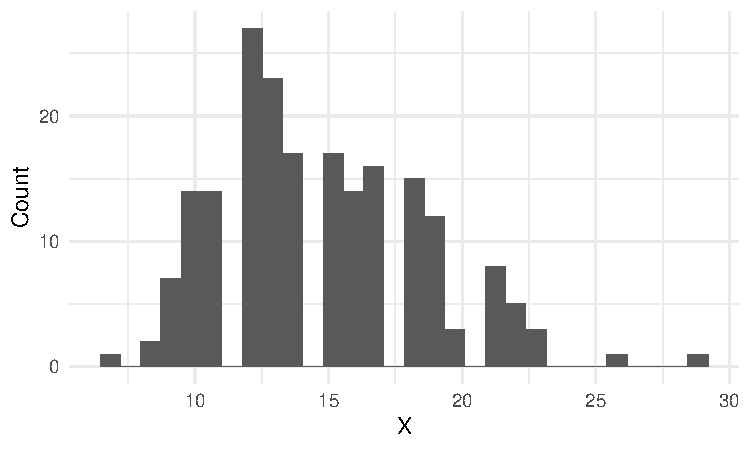
\includegraphics[width=\maxwidth]{img/mc-distribution-02-a-1} 

}







\begin{enumerate}
\item [\textbf{A} \msquare] Es handelt sich um eine Poisson-Verteilung mit Pois(15).
\item [\textbf{B} \msquare] Eine rechtsschiefe, multivariate Normalverteilung.
\item [\textbf{C} \msquare] Es handelt sich um eine Binomial-Verteilung mit Binom(10).
\item [\textbf{D} \msquare] Es handelt sich um eine Normalverteilung mit N(15, 5).
\item [\textbf{E} \msquare] Eine Standardnormalverteilung mit N(0,1).
\end{enumerate}

% -----------------------------------------------------------------------
\clearpage
% -----------------------------------------------------------------------

\section{Aufgabe \hfill (10 Punkte)}

\textit{Geben Sie grunds{\"a}tzlich Formeln und Rechenweg zur L{\"o}sung der
  Teilaufgaben mit an!} \\[1Ex]

%% --------------------------------------------------------------------
\hfill\href{https://youtu.be/VAqiUdV4WQ0}{
\includegraphics[width =
  2cm]{img/youtube}}\\[1Ex]
%% --------------------------------------------------------------------

In einem Feldexperiment f{\"u}r die Bodendurchl{\"a}ssigkeit wurde der Niederschlag
pro Parzelle sowie der durchschnittliche Ertrag gemessen. Es ergibt sich
folgende Datentabelle. 

\begin{table}[!h]
\centering
\begin{tabular}{cc}
\toprule
water & drymatter\\
\midrule
25 & 24\\
22 & 20\\
25 & 20\\
24 & 23\\
25 & 21\\
\addlinespace
25 & 19\\
25 & 21\\
24 & 20\\
23 & 21\\
\bottomrule
\end{tabular}
\end{table}



\begin{enumerate}
\item Erstellen Sie den Scatter-Plot f{\"u}r die Datentabelle. Beschriften Sie
  die Achsen entsprechend! \textbf{(4 Punkte)}
\item Zeichnen Sie eine Gerade durch die Punkte! \textbf{(1 Punkt)}
\item Beschriften Sie die Gerade mit den g{\"a}ngigen statistischen Ma{\ss}zahlen!
  Geben Sie die numerischen Zahlenwerte mit an! \textbf{(3 Punkte)}
\item Wenn kein Effekt von dem Niederschlag auf das Trockengewicht
  vorhanden w{\"a}re, wie w{\"u}rde die Gerade verlaufen und welche Werte w{\"u}rden die
  statistischen Ma{\ss}zahlen annehmen? \textbf{(2 Punkt)}
\end{enumerate} 
\clearpage
% -----------------------------------------------------------------------

\section{Aufgabe \hfill (8 Punkte)}

\textit{Geben Sie grunds{\"a}tzlich Formeln und Rechenweg zur L{\"o}sung der
  Teilaufgaben mit an!} \\[1Ex]

%% --------------------------------------------------------------------
 \hfill\href{https://youtu.be/hr_jPd1hpKY}{
\includegraphics[width =
   2cm]{img/youtube}}\\[1Ex]
%% --------------------------------------------------------------------


In einem Experiment zur Dosiswirkung wurden verschiedene Dosisstufen mit
einer Kontrollgruppe vergleichen. Es wurden verschiedene t-Test f{\"u}r den
Mittelwertsvergleich gerechnet und es ergab sich folgende Tabelle mit den
rohen p-Werten (\textit{Raw p-value}).


\begin{knitrout}
\definecolor{shadecolor}{rgb}{0.969, 0.969, 0.969}\color{fgcolor}\begin{table}[!h]
\centering\begingroup\fontsize{12}{14}\selectfont

\begin{tabular}{cccc}
\toprule
Vergleich & Raw p-value & Adjusted p-value & Reject Null\\
\midrule
dose 25 - ctrl & 0.0300 &  & \\
dose 30 - ctrl & 0.3400 &  & \\
dose 60 - ctrl & 0.0012 &  & \\
dose 50 - ctrl & 0.0800 &  & \\
\bottomrule
\end{tabular}
\endgroup{}
\end{table}

\end{knitrout}


%\begin{center}
%  \Large
%  \begin{tabular}{c|c|c|c}
%    \textbf{Vergleich} & \textbf{Raw p-val} & \textbf{Adjusted p-val} &
%                                                                        \textbf{Reject $\boldsymbol{H_0}$} \strut\\
%    \hline
%    dose 10 - ctrl  & pval_vec[1] &  &\strut\\
%    \hline
%    dose 15 - ctrl  & pval_vec[2] & &\strut\\
%    \hline
%    dose 20 - ctrl  & pval_vec[3] & &\strut\\
%    \hline
%    dose 40 - ctrl  & pval_vec[4] & &\strut\\
%  \end{tabular}
%\end{center}

\begin{enumerate}
\item F{\"u}llen Sie die Spalte "`Adjusted p-value"' mit den adjustierten
  p-Werten nach Bonferoni aus! \textbf{(4 Punkte)}
\item Entscheiden Sie, ob nach der Adjustierung die Nullhypothese weiter
  abgelehnt werden kann. Tragen Sie Ihre Entscheidung in die obige Tabelle
  ein. Begr{\"u}nden Sie Ihre Antwort! \textbf{(2 Punkte)}
\item Erkl{\"a}ren Sie warum die p-Werte bei multiplen Vergleichen
  adjustiert werden m{\"u}ssen! \textbf{(2 Punkte)}
\end{enumerate}

\vspace{1Ex}

 
\clearpage
% -----------------------------------------------------------------------

\section{Aufgabe \hfill (13 Punkte)}

\textit{Geben Sie grunds{\"a}tzlich Formeln und Rechenweg zur L{\"o}sung der
  Teilaufgaben mit an!} \\[1Ex]

%% --------------------------------------------------------------------
\hfill\href{https://youtu.be/49hvImMwVyE}{
\includegraphics[width =
  2cm]{img/youtube}}\\[1Ex]
%% --------------------------------------------------------------------


Der Datensatz \texttt{plant\_growth\_tbl} enth{\"a}lt das Gewicht der Kohlk{\"o}pfe
(\textit{weight}), die unter einer Kontrolle und zwei verschiedenen
Behandlungsbedingungen erzielt wurden -- dem Faktor \textit{group} mit den
Faktorstufen \textit{ctrl}, \textit{trt1}, \textit{trt2}.



\begin{enumerate}
\item F{\"u}llen Sie die unterstehende einfaktorielle ANOVA Ergebnistabelle aus
  mit den gegebenen Informationen von \texttt{Df} und \texttt{Sum Sq}!
  \textbf{(4 Punkte)}
\item Sch{\"a}tzen Sie den p-Wert der Tabelle mit der Information von
  $F_{\alpha = 5\%} = 3.49$ ab. Begr{\"u}nden Sie Ihre
  Antwort! \textbf{(2 Punkte)}
\end{enumerate}

\vspace{1Ex}

\begin{center}
  \Large
  \begin{tabular}{l|c|c|c|c|c}
     & \textbf{Df} & \textbf{Sum Sq} & \textbf{Mean Sq} & \textbf{F value} & \textbf{Pr(>F)} \strut\\
    \hline
   \textbf{group}  & 2 & 232.49 &  &  &  \strut\\
    \hline
   \textbf{Residuals}  & 20 & 48.98 &  &  &  \strut\\
  \end{tabular}
\end{center}

\vspace{1Ex}

\begin{enumerate}
  \setcounter{enumi}{2}
\item Was bedeutet ein signifikantes Ergebnis in einer einfaktoriellen
  ANOVA im Bezug auf die m{\"o}glichen Unterschiede zwischen den Gruppen? Beziehen Sie sich auf den obigen Fragetext bei Ihrer Antwort!
  \textbf{(2 Punkte)}
\item Berechnen Sie \textit{einen} Student t-Test mit f{\"u}r den \textit{vermutlich}
  signifikantesten Gruppenvergleich anhand der untenstehenden Tabelle mit
  $T_{\alpha = 5\%} = 2.03$. Begr{\"u}nden Sie Ihre Auswahl! \textbf{(3 Punkte)}
\end{enumerate}

\begin{knitrout}
\definecolor{shadecolor}{rgb}{0.969, 0.969, 0.969}\color{fgcolor}\begin{table}[!h]
\centering
\begin{tabular}{cccc}
\toprule
group & n & mean & sd\\
\midrule
ctrl & 7 & 14.43 & 1.13\\
trt1 & 9 & 18.78 & 1.72\\
trt2 & 7 & 22.57 & 1.72\\
\bottomrule
\end{tabular}
\end{table}

\end{knitrout}

\begin{enumerate}
  \setcounter{enumi}{4}
\item Gegebenen der ANOVA Tabelle war das Ergebnis des t-Tests zu erwarten?
  Begr{\"u}nden Sie Ihre Antwort! \textbf{(2 Punkte)}
\end{enumerate}

 
\clearpage
% -----------------------------------------------------------------------

\section{Aufgabe \hfill (7 Punkte)}

\textit{Geben Sie grunds{\"a}tzlich Formeln und Rechenweg zur L{\"o}sung der
  Teilaufgaben mit an!} \\[1Ex]

%% --------------------------------------------------------------------
\hfill\href{https://youtu.be/vXnLttRL_VI}{
\includegraphics[width =
  2cm]{img/youtube}}\\[1Ex]
%% --------------------------------------------------------------------



In einem Gew{\"a}chshausexperiment mit drei Substrattypen ($torf$, $40p60n$ und $70p30n$) als Behandlung
(\textit{treatment}) ergibt sich die folgende Datentabelle mit dem
gemessenen Frischgewicht (\textit{freshmatter}) von Maiss.

\begin{table}[!h]
\centering
\begin{tabular}{cc}
\toprule
treatment & freshmatter\\
\midrule
70p30n & 27.7\\
torf & 41.0\\
40p60n & 15.9\\
70p30n & 27.5\\
torf & 35.9\\
\addlinespace
40p60n & 26.4\\
70p30n & 29.8\\
torf & 40.2\\
40p60n & 21.8\\
\bottomrule
\end{tabular}
\end{table}



\begin{enumerate}
\item Zeichnen Sie in \textit{einer} Abbildung die Barplots f{\"u}r die
  Behandlung von Maiss! Beschriften Sie die Achsen entsprechend!
  \textbf{(4 Punkte)}
\item Beschriften Sie \textit{einen} Barplot mit den g{\"a}ngigen
  statistischen Ma{\ss}zahlen! \textbf{(2 Punkte)}
\item Wenn Sie \textit{keinen Effekt} zwischen den Behandlungen von
  Maiss erwarten w{\"u}rden, wie sehen dann die Barplots aus?
  \textbf{(1 Punkt)}
\end{enumerate} 
\clearpage
% -----------------------------------------------------------------------

\section{Aufgabe \hfill (10 Punkte)}

\textit{Geben Sie grunds{\"a}tzlich Formeln und Rechenweg zur L{\"o}sung der
  Teilaufgaben mit an!} \\[1Ex]

%% --------------------------------------------------------------------
\hfill\href{https://youtu.be/lJp8rFmMnrs}{
\includegraphics[width =
  2cm]{img/youtube}}\\[1Ex]
%% --------------------------------------------------------------------



In einem Stallexperiment mit $n = 120$ Ferkeln wurde der
Gewichtszuwachs in kg unter ansteigender Lichteinstrahlung in nm
gemessen. Sie erhalten den \Rlogo Output einer
simplen Gaussian linearen Regression sieben Wochen nach der ersten Messung.

\begin{table}[!h]
\centering\begingroup\fontsize{14}{16}\selectfont

\begin{tabular}{ccccc}
\toprule
term & estimate & std.error & t statistic & p-value\\
\midrule
(Intercept) & 1.69 & 1.22 &  & \\
light & 1.01 & 0.12 &  & \\
\bottomrule
\end{tabular}
\endgroup{}
\end{table}



\begin{enumerate}
\item Berechnen Sie die t Statistik f{\"u}r \textit{(Intercept)} und
  \textit{light}! \textbf{(2 Punkte)}
\item Sch{\"a}tzen Sie den p-Wert f{\"u}r \textit{(Intercept)} und
  \textit{light} mit $T_{\alpha = 5\%} = 1.96$ ab. Was sagt Ihnen der p-Wert aus?
  Begr{\"u}nden Sie Ihre Antwort! \textbf{(3 Punkte)}
\item Zeichnen Sie die Grade aus der obigen Tabelle in ein Koordinatenkreuz! \textbf{(1 Punkt)}
\item Beschriften Sie die Abbildung und die Gerade mit den statistischen
  Kenngr{\"o}{\ss}en! \textbf{(2 Punkte)}
\item Formulieren Sie die Regressionsgleichung! \textbf{(2 Punkte)}
\end{enumerate} 
\clearpage
% -----------------------------------------------------------------------

\section{Aufgabe \hfill (10 Punkte)}

%% --------------------------------------------------------------------
\hfill\href{https://youtu.be/exDo7AyHl4Q}{
\includegraphics[width =
  2cm]{img/youtube}}\\[1Ex]
%% --------------------------------------------------------------------

Sie erhalten folgende \Rlogo Ausgabe der Funktion \texttt{t.test()}.

\begin{knitrout}
\definecolor{shadecolor}{rgb}{0.969, 0.969, 0.969}\color{fgcolor}\begin{kframe}
\begin{verbatim}
## 
## 	Two Sample t-test
## 
## data:  waterintake by infusion
## t = -2.1373, df = 10, p-value = 0.0583
## alternative hypothesis: true  is not equal to [condensed]
## 95 percent confidence interval:
##  -5.9524618  0.1238903
## sample estimates:
##  mean in group mid mean in group trt2 
##           13.28571           16.20000
\end{verbatim}
\end{kframe}
\end{knitrout}


\begin{enumerate}
  \item Formulieren Sie das statistische Hypothesenpaar! \textbf{(2
Punkte)}
\item Liegt ein signifikanter Unterschied zwischen den Gruppen vor?
  Begr{\"u}nden Sie Ihre Antwort! \textbf{(2 Punkte)}
\item Skizieren Sie eine Abbildung in der Sie $T_{calc}$, $Pr(D|H_0)$, $A=0.95$,
  sowie $T_{\alpha=5\%} = |2.23|$ einzeichnen! \textbf{(4 Punkte)}
\item Beschriften Sie die Abbildung entsprechend! \textbf{(2 Punkte)}  
\end{enumerate} 
\clearpage
% -----------------------------------------------------------------------

\section{Aufgabe \hfill (9 Punkte)}

%% --------------------------------------------------------------------
\hfill\href{https://youtu.be/32JjH1eyuTU}{
\includegraphics[width =
  2cm]{img/youtube}}\\[1Ex]
%% --------------------------------------------------------------------



Im Folgenden ist die t-Verteilung unter der Anahme der G{\"u}ltigkeit der
Nullhypothese abgebildet. 

\begin{enumerate}
\item Erg{\"a}nzen Sie die Beschriftung der $x$-Achse! \textbf{(1 Punkt)}
\item Erg{\"a}nzen Sie "`$\bar{y}_1 = \bar{y}_2$"'! \textbf{(1 Punkt)} 
\item Erg{\"a}nzen Sie "`$A = 0.95$"'! \textbf{(1 Punkt)}
\item Zeichnen Sie $T_{\alpha=5\%}$ in die Abbildung! \textbf{(1 Punkt)} 
\item Zeichnen Sie das Signifikanzniveau $\alpha$ in die Abbildung! \textbf{(2 Punkte)} 
\item Zeichnen Sie $+T_{calc}$ in die Abbildung! \textbf{(1
    Punkt)}
\item Zeichnen Sie einen nicht signifikant p-Wert in die Abbildung! \textbf{(2 Punkte)}   
\end{enumerate}



{\centering 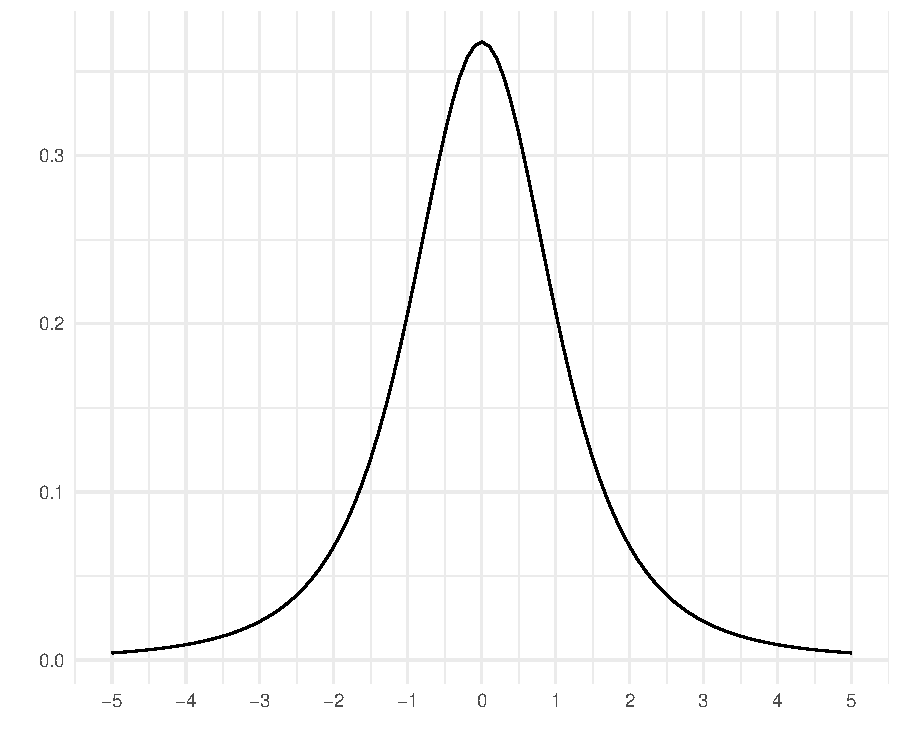
\includegraphics[width=\maxwidth]{img/statistisches-testen-3-1} 

}


 
\clearpage
% -----------------------------------------------------------------------
\end{document}
% -----------------------------------------------------------------------


  
